\chapter{Data analysis}
\label{cha:data_analysis}

\section{Data acknowledgements}

Due to data usage legal restrictions and Ericsson's customers' privacy, internal identifiers used by the company's operations and dates in all timestamps have been anonymised in the thesis available for the public domain. Moreover, the data structures and sensitive data values have not been presented.

\section{Data description}
\label{sec:data_description}

The available data is in the form of time series indexed by an \ac{rbs} unique identifier and the time stamp corresponding to sample time. The data is sparse and in different files depending on the domains from where the features have been measured, i.e., the power supply, power distribution, radio traffic, cabinet climate, etc. A brief explanation of the information provided by the time series and some random samples from the database are shown in the following subsections. It should be noted that configuration data for base stations is included. This data shows hardware equipment and their settings, for example, the number of \acp{psu}. 

\subsection{Power supply}
\label{subsec:data_description:power_supply}

\subsubsection*{Power supply interruptions from the Power Grid distribution}

This measurement shows how stable the electric power supply from the AC distribution is, i.e., it is a time counter in which the energy supply has been interrupted from the public power distribution. 
As a consequence, \ac{rbs} utilise power from other sources such as batteries.

\subsubsection*{\ac{psu} utilisation statistics}

\ac{psu} utilisation refers to the percentage of \ac{psu}'s power capacity being consumed by the loads over a determined time. In the available data for this project, this is described by the average, minimum, maximum and standard deviation of these measures over different time durations.

These statistics are, in fact, the most crucial feature in the present work. It can be understood as the complement of the power headroom in per cent. In order to obtain the power values in terms of Watt, the installed power capacity needs to be known. 

As there are no direct power headroom measurements, the \ac{psu} utilisation has been chosen as the target variable, and then the power headroom will be derived from this quantity. In the Figure \ref{fig:feats_avgpsu}, the average of a \ac{psu} utilisation is shown as an example. 

\begin{figure}[hptb]
	\centering
	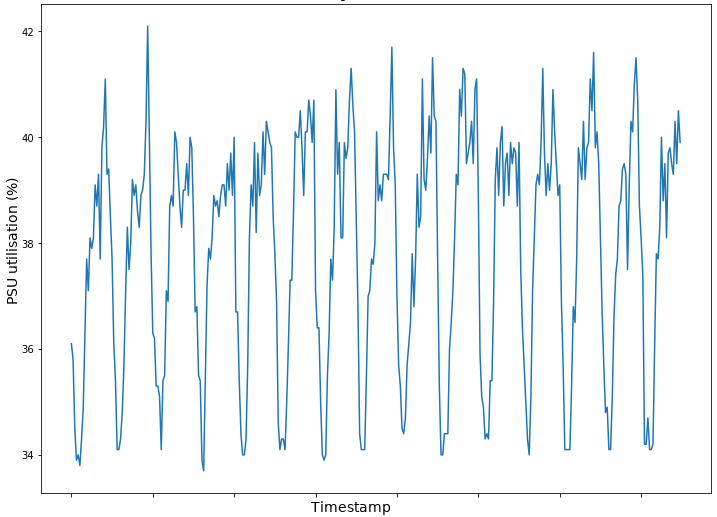
\includegraphics[width=0.65\textwidth]{avg_psu_utilization}
	\caption{Average PSU utilisation example}
	\label{fig:feats_avgpsu}
\end{figure}


\subsection{Radio energy}

\subsubsection*{Radio units voltage statistics}

The \acp{ru} are fed with energy by the \ac{pdu}. Nonetheless, this is not constant and might change over time. The minimum, maximum, average and standard deviation statistics show how these fluctuations have been over a determined time. Figure \ref{fig:feats_std_ru_voltage} shows the standard deviation of the voltage perceived by the \acp{ru}. 

\begin{figure}[hptb]
	\centering
	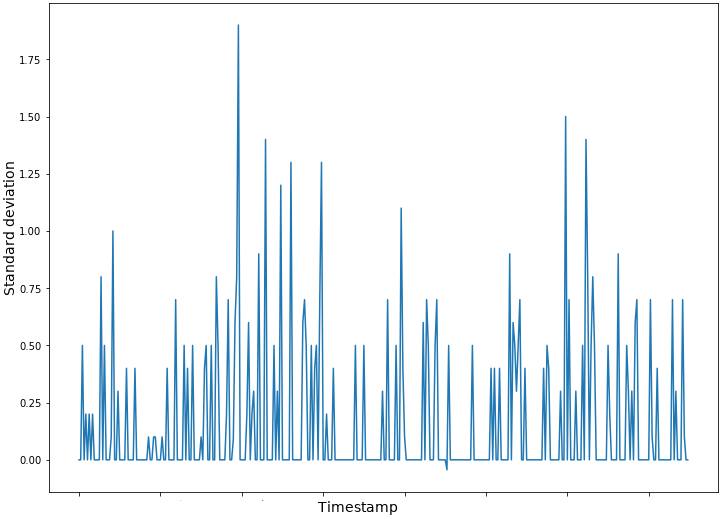
\includegraphics[width=0.65\textwidth]{std_ru_voltage}
	\caption{Standard deviation of \ac{ru} voltage example}
	\label{fig:feats_std_ru_voltage}
\end{figure}

\subsubsection*{Radio units power consumption statistics}

Supplied energy and power consumption are not the same. Whereas the former refers to the available energy to be used, the consumed power refers to the actual power used for broadcasting purposes. The minimum, maximum, average and standard deviation statistics have been measured and reported over a determined time. Figure \ref{fig:feats_avg_ru_power_consumption} presents the average of the consumed power by the \ac{ru} as an example.

\begin{figure}[hptb]
	\centering
	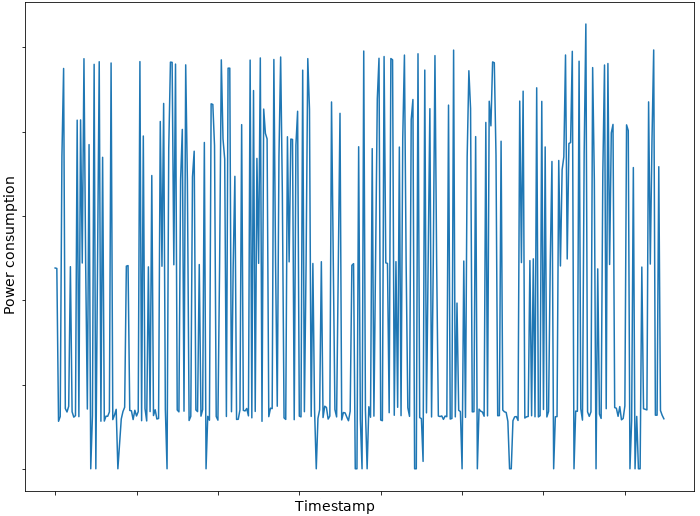
\includegraphics[width=0.65\textwidth]{avg_ru_power_consumption}
	\caption{Average \ac{ru} power consumption example}
	\label{fig:feats_avg_ru_power_consumption}
\end{figure}

\subsection{Power distribution}

As shown in Figure \ref{fig:powerinfrastucture}, the \acp{ru} are not fed directly by the \acp{psu} but by the \ac{pdu} which manages the different power sources of the \ac{rbs}. The measurements in the \ac{pdu} do not need to be the same as the voltage and power measurements in the \acp{ru} because the power lines that connect them could be up to 60 metres long, which might introduce some losses to the system.

Like other features, these are sampled and presented as their minimum, maximum, average and standard deviation over a determined time. Figure \ref{fig:feats_avg_pdu_voltage} shows the average of the \ac{pdu}'s output voltage as example.

\begin{figure}[hptb]
	\centering
	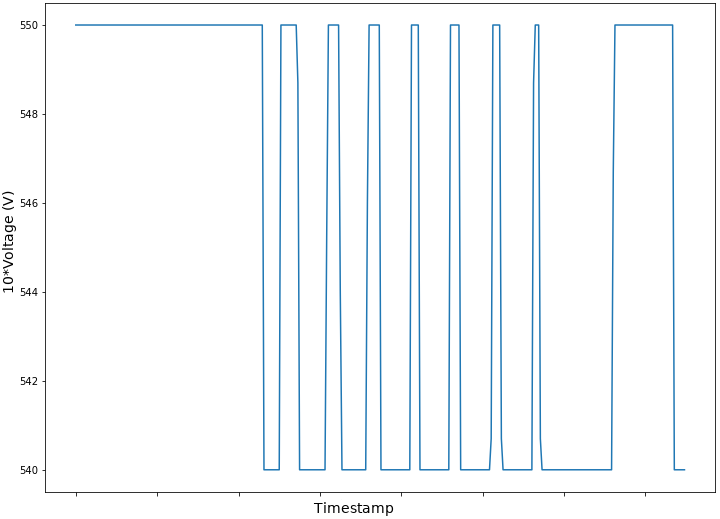
\includegraphics[width=0.65\textwidth]{avg_pdu_voltage}
	\caption{Average \ac{pdu} voltage example}
	\label{fig:feats_avg_pdu_voltage}
\end{figure}


\subsection{Radio traffic}

In the data measured from radio traffic, it is possible to observe the highly seasonal characteristics of users behaviour influenced by the day-night cycle. Examples of data are shown in Figures \ref{fig:feats_connections}. \ref{fig:feats_data_blocks}, and \ref{fig:feats_active_users}. 

\subsubsection*{Number of connections}

This measurement corresponds to the number of established connections to the radio traffic.

\begin{figure}[H]
	\centering
	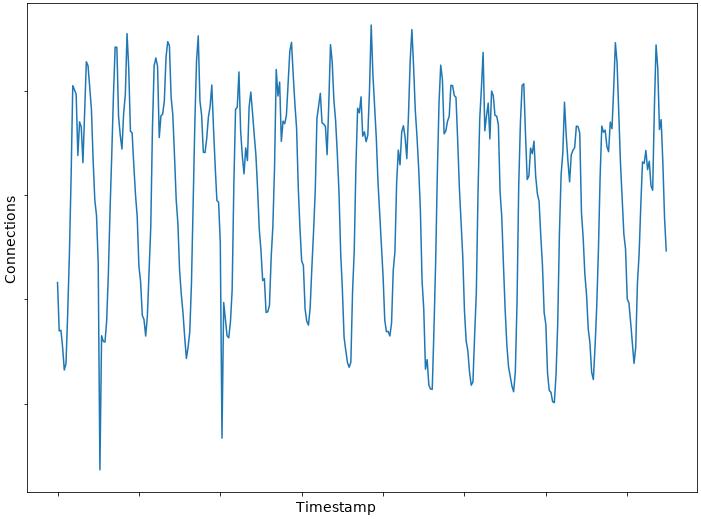
\includegraphics[width=0.65\linewidth]{connections.png}
	\caption{Connections requests signal example}
	\label{fig:feats_connections}
\end{figure}

\subsubsection*{Data blocks}

This signal corresponds to the number of resource blocks connected to the traffic load in the uplink and downlink.

\begin{figure}[H]
	\centering
	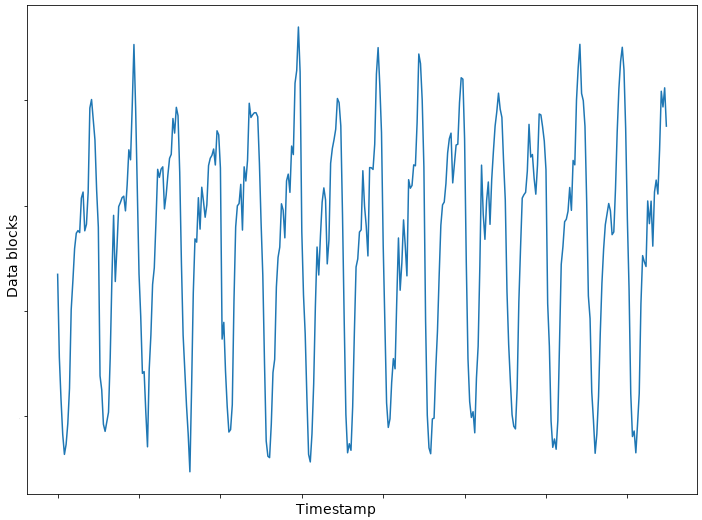
\includegraphics[width=0.65\linewidth]{data_blocks.png}
	\caption{Data blocks signal example}
	\label{fig:feats_data_blocks}
\end{figure}

\pagebreak
\subsubsection*{Active Users}

This feature shows the number of active users connected to the radio traffic load in the uplink and downlink.

\begin{figure}[H]
	\centering
	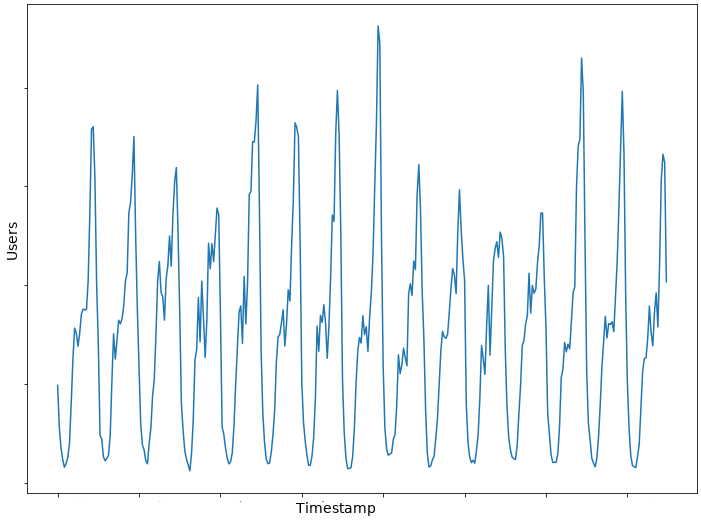
\includegraphics[width=0.65\linewidth]{active_users.png}
	\caption{Active users signal example}
	\label{fig:feats_active_users}
\end{figure}


\subsection{Climate}

\subsubsection*{Average cabinet temperature}

In electronic components, high temperature is highly correlated with power dissipation; therefore, its increments in the hardware units will also increase the temperature within the cabinet. An example of average cabinet temperature time series is shown in Figure \ref{fig:feats_cabinet_temp}. 

\begin{figure}[H]
	\centering
	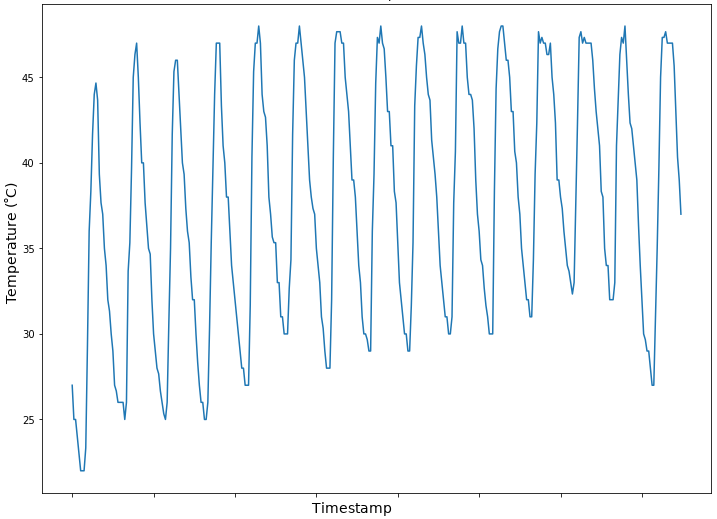
\includegraphics[width=0.65\linewidth]{cabinet_temp.png}
	\caption{Cabinet temperature signal example}
	\label{fig:feats_cabinet_temp}
\end{figure}

\pagebreak
\subsubsection*{Internal and external fan speed}

The cabinet is designed to keep the hardware safe. When the cabinet temperature is considered \emph{high}, the fans, one internal and the other external, will be managed to cool down the hardware units. Therefore, the higher the temperature, the faster the fans will run. The reported values correspond to percentages of possible speed values, i.e.,  a zero value represents a steady fan, whereas a 100 means maximum velocity. Internal and external fan speed signals are shown in Figure \ref{fig:feats_int_fan} and \ref{fig:feats_ext_fan}.

\begin{figure}[hptb]
	\begin{subfigure}{.47\textwidth}
		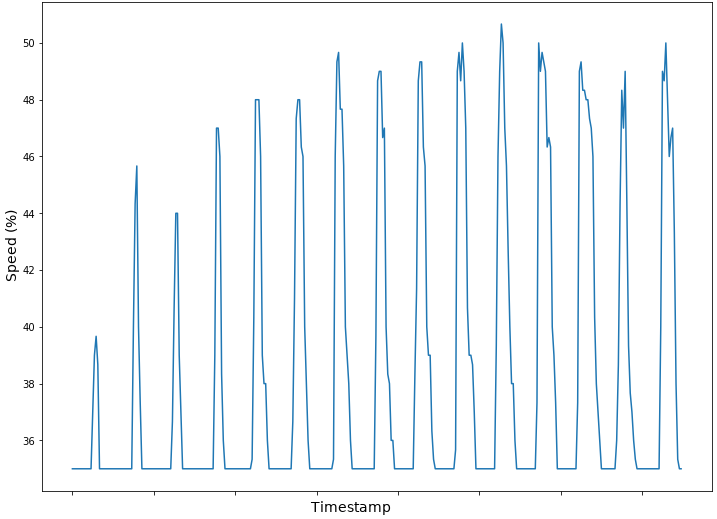
\includegraphics[width=\textwidth]{internal_fan}
		\caption{Internal fan speed}
		\label{fig:feats_int_fan}
	\end{subfigure}%
	\hfill
	\begin{subfigure}{.47\textwidth}
		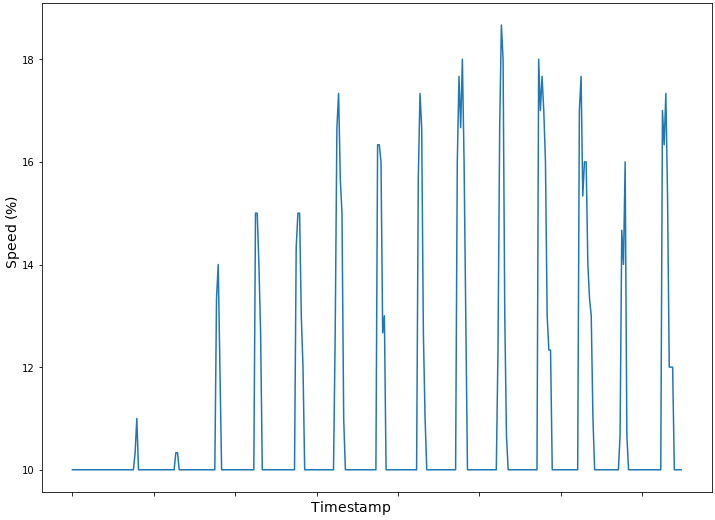
\includegraphics[width=\textwidth]{external_fan}
		\caption{External fan speed}
		\label{fig:feats_ext_fan}
	\end{subfigure}
	\caption{Internal and external fan speed signals examples}
\end{figure}

